\documentclass[14pt,a4paper]{scrartcl}
\usepackage{cmap}
\usepackage[utf8]{inputenc}
\usepackage[T1,T2A]{fontenc}
\usepackage[english,russian]{babel}
\usepackage{relsize}
\usepackage{graphicx}
\usepackage{subfigure}
\usepackage{mathtools}
\usepackage{amssymb}
\usepackage{float}
\usepackage{sidecap}
\usepackage{wrapfig}
\usepackage{caption}
\usepackage[table,xcdraw]{xcolor}
\usepackage{listings}
\usepackage{amsmath,cryptocode}
\usepackage{listings}
\usepackage{booktabs}
\usepackage{multirow}  
\usepackage{multicol}
\usepackage{bigstrut}
\usepackage{lscape}
\usepackage{rotating}
\usepackage{adjustbox}
\usepackage{minted}
\usepackage{breqn}
\usepackage{physics}


\newcommand\scalemath[2]{\scalebox{#1}{\mbox{\ensuremath{\displaystyle #2}}}}


\begin{document}
	\begin{titlepage}
	\begin{center}
		\large
		МИНИСТЕРСТВО ОБРАЗОВАНИЯ И НАУКИ\\ РОССИЙСКОЙ ФЕДЕРАЦИИ
		
		\vspace{0.5cm}
		
		МГТУ им Н.Э.Баумана
		\vspace{0.25cm}
		
		Факультет ФН
		
		Кафедра вычислительной математики и математической физики
		\vfill
		
		
		Соколов Арсений Андреевич\\
		\vfill
		
		
		{\LARGE Лабораторная работа №8 по численным методам\\[2mm]
		}
		\bigskip
		
		3 курс, группа ФН11-53Б\\
		Вариант 6
	\end{center}
	\vfill
	
	\newlength{\ML}
	\settowidth{\ML}{«\underline{\hspace{0.7cm}}» \underline{\hspace{2cm}}}
	\hfill\begin{minipage}{0.4\textwidth}
		Преподаватель\\
		\underline{\hspace{3cm}} В.\,А.~Кутыркин\\
		«\underline{\hspace{0.7cm}}» \underline{\hspace{1.71cm}} 2019 г.
	\end{minipage}%
	\bigskip
	
	
	\vfill
	
	\begin{center}
		Москва, 2019 г.
	\end{center}
\end{titlepage}

\section*{Задание 1}
\textbf{Задание.}\\
Для заданной на отрезке $[0;2]$ гладкой функции $f(x)=\frac{(a+52-n) x^{4}+(b-51+n) x^{2}+c}{(x+1)\left(x^{2}+1\right)}$, где $N$ -- номер студента в журнале, $n$ -- номер группы, и равномерной сетки $A = \langle \tau_0, \tau_1, \ldots, \tau_k \rangle$, где $k = 20$, используя квадратурные формулы прямоугольников, трапеций и парабол, приближённо вычислить интеграл $\int_{0}^{2}f(\tau)d\tau$.\\
Прокомментировать приближённые результаты, сравнивая их с
аналитически вычисленным значением интеграла


\textbf{Исходные данные.}\\
$N = 6, n = 53, a = 3, b = 6, c = 1$

\begin{equation*}
	\frac{(3 + 52 - 53)x^4 + (6-51+53)x^2 + 1}{(x+1)(x^2+1)} = \frac{1 + 8 x^2 + 2 x^4}{(1 + x) (1 + x^2)}
\end{equation*}

\textbf{Решение.}\\
На отрезке $[0;2]$ задана равномерная сетка $A = \langle \tau_0, \tau_1, \ldots, \tau_k \rangle$, где $k=20$, с шагом $\frac{b-a}{k} = 0.1$.

Получаем:
\begin{equation*}
	A=\left\langle 0, \frac{1}{10}, \frac{1}{5}, \frac{3}{10}, \frac{2}{5}, \frac{1}{2}, \frac{3}{5}, \frac{7}{10}, \frac{4}{5}, \frac{9}{10},1, \frac{11}{10}, \frac{6}{5}, \frac{13}{10}, \frac{7}{5}, \frac{3}{2}, \frac{8}{5}, \frac{17}{10}, \frac{9}{5},\frac{19}{10}, 2\right\rangle
\end{equation*}

Квадратурная формула прямоугольников:
\begin{equation*}
	\int_{0}^{2} f(\tau) d \tau=h\left(f\left(\theta_{1}\right)+\ldots+f\left(\theta_{2} 0\right)\right)+O(h) \textup{при } h \rightarrow 0,
\end{equation*}
где $\theta_{1} = \frac{\tau_0 + \tau_1}{2}, \ldots, \theta_{20} = \frac{\tau_{19} + \tau_{20}}{2}$ -- центрально-равномерная сетка отрезка $[0;2]$.

Получаем:
\begin{equation*}
	\left\langle\frac{1}{20}, \frac{3}{20}, \frac{1}{4}, \frac{7}{20}, \frac{9}{20}, \frac{11}{20}, \frac{13}{20}, \frac{3}{4}, \frac{17}{20}, \frac{19}{20}, \frac{21}{20}, \frac{23}{20}, \frac{5}{4}, \frac{27}{20}, \frac{29}{20}, \frac{31}{20}, \frac{33}{20}, \frac{7}{4}, \frac{37}{20}, \frac{39}{20}\right\rangle
\end{equation*}

\begin{equation*}
\int_{0}^{2} f(\tau) d \tau=h\left(f\left(\theta_{1}\right)+\ldots+f\left(\theta_{2} 0\right)\right)+O(h) = 5.285262010,
\end{equation*}

Квадратурная формула трапеции:
\begin{equation*}
	\int_{0}^{2} f(\tau) d \tau=h\left(\frac{1}{2} f\left(\tau_{0}\right)+f\left(\tau_{1}\right)+\ldots+f\left(\tau_{19}\right)+\frac{1}{2} f\left(\tau_{20}\right)\right)+O\left(h^{2}\right) \textup{при } h \rightarrow 0
\end{equation*}

Получаем:

\begin{equation*}
\int_{0}^{2} f(\tau) d \tau=h\left(\frac{1}{2} f\left(\tau_{0}\right)+f\left(\tau_{1}\right)+\ldots+f\left(\tau_{19}\right)+\frac{1}{2} f\left(\tau_{20}\right)\right)+O\left(h^{2}\right) = 5.288360556
\end{equation*}

Квадратурная формула парабол:\\
Если $k$ -- чётное, то
\begin{equation*}\resizebox{1 \textwidth}{!} 
{
	$
	\int_{0}^{2} f(\tau) d \tau=\frac{h}{3}\left(f\left(\tau_{0}\right)+4 f\left(\tau_{1}\right)+2 f\left(\tau_{2}\right)+4 f\left(\tau_{3}\right)+\ldots+2 f\left(\tau_{18}\right)+4 f\left(\tau_{19}\right)+f\left(\tau_{20}\right)\right)+O\left(h^{3}\right), \textup{при } h \rightarrow 0$}
\end{equation*}

Получаем:
\begin{equation*}\resizebox{1 \textwidth}{!} 
{
	$
	\int_{0}^{2} f(\tau) d \tau=\frac{h}{3}\left(f\left(\tau_{0}\right)+4 f\left(\tau_{1}\right)+2 f\left(\tau_{2}\right)+4 f\left(\tau_{3}\right)+\ldots+2 f\left(\tau_{18}\right)+4 f\left(\tau_{19}\right)+f\left(\tau_{20}\right)\right)+O\left(h^{3}\right) = 5.286319825$}
\end{equation*}

Вычислим аналитическое значение интеграла:
\begin{equation*}
	\int_{0}^{2} {\frac {2\,{x}^{4}+8\,{x}^{2}+1}{ \left( x+1 \right)  \left( {x}^{2}+1
			\right) }} = \frac{1}{4} (22 \log(3) + 5\log(5) - 10 \atan(2))
	 \approx 5.286293185 
\end{equation*}

\textbf{Результат.}\\
Рассмотрим модули разностей полученных решений тремя способами со значением интеграла, вычисленного аналитически:
\begin{figure}[H]
	\begin{minipage}[h]{1\linewidth}
		\center{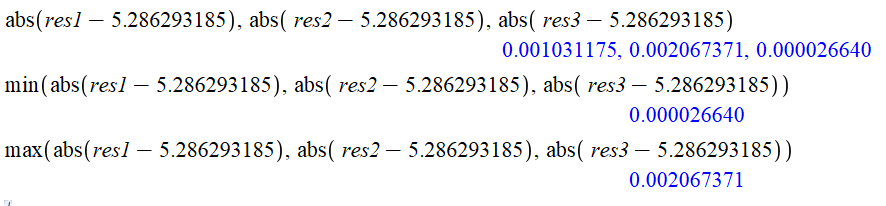
\includegraphics[width=1\linewidth]{../img/img1.png}}  \\
	\end{minipage}
\end{figure}


Видим, что наибольшую точность даёт квадратурная формула трапеции, а наименьшую точность -- квадратурная формула парабол.

\end{document}